\documentclass[tikz,border=2pt]{standalone}
\usepackage{amsmath,amssymb,bm}
\usepackage[scaled=0.92]{helvet}
\usetikzlibrary{arrows.meta,positioning,fit,calc,backgrounds}

% stream colors: common (blue), private (gray), multicast (purple)
\definecolor{cfill}{HTML}{DCE6F4}
\definecolor{cedge}{HTML}{2F4A73}
\definecolor{pfill}{HTML}{EEEEEE}
\definecolor{pedge}{HTML}{4D4D4D}
\definecolor{mcol}{HTML}{7A3E8E}
\definecolor{grp}{HTML}{8C8C8C}
\definecolor{txfill}{HTML}{F4F6FA}
\definecolor{rxfill}{HTML}{F7F5F0}

\begin{document}
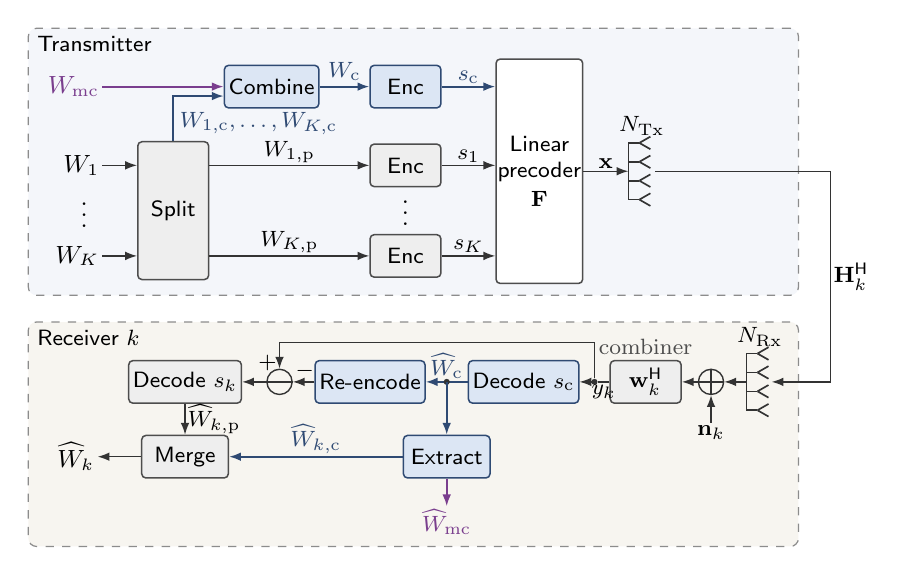
\begin{tikzpicture}[
    font=\small,
    >={Latex[length=1.5mm,width=1.1mm]},
    line/.style={draw=black!80, line width=0.5pt},
    cline/.style={draw=cedge, line width=0.7pt},
    mline/.style={draw=mcol, line width=0.7pt},
    blk/.style={draw=pedge, line width=0.55pt, fill=pfill, rounded corners=1.5pt,
                minimum height=5.4mm, inner sep=1.5pt, font=\sffamily\footnotesize,
                align=center},
    cblk/.style={blk, draw=cedge, fill=cfill},
    lab/.style={font=\fontsize{9.2}{11}\selectfont, inner sep=1pt},
    sm/.style={font=\fontsize{8.2}{10}\selectfont, inner sep=0.8pt},
    grpbox/.style={draw=grp, dashed, line width=0.45pt, rounded corners=3pt, inner sep=4pt},
    txbg/.style={grpbox, fill=txfill},
    rxbg/.style={grpbox, fill=rxfill},
    grplab/.style={font=\sffamily\footnotesize, text=black, inner sep=1pt},
    sum/.style={circle, draw=black!80, line width=0.5pt, inner sep=0pt, minimum size=3.2mm},
    dot/.style={circle, fill=black!80, inner sep=0pt, minimum size=2.2pt},
]

% ================= transmitter =================
\def\xL{-0.55}   % common left edge of both boxes
\def\xR{8.95}    % common right edge of both boxes
\def\yC{0.75}     % common branch
\def\yA{-0.25}    % private branch of user 1
\def\yK{-1.4}    % private branch of user K

% messages
\node[lab, anchor=east, text=mcol] (wmc) at (0.25,\yC) {$W_{\mathrm{mc}}$};
\node[lab, anchor=east] (w1) at (0.25,\yA) {$W_1$};
\node[lab, anchor=east] (wK) at (0.25,\yK) {$W_K$};
\node[lab] at (0.02,{(\yA+\yK)/2+0.05}) {$\vdots$};

% rate splitting
\node[blk, minimum width=9mm, minimum height=17.5mm] (split) at (1.15,{(\yA+\yK)/2}) {Split};
\draw[line,->] (w1) -- (w1 -| split.west);
\draw[line,->] (wK) -- (wK -| split.west);

% combiner of the common parts and the multicast message
\node[cblk, minimum width=12mm] (comb) at (2.4,\yC) {Combine};
\draw[mline,->] (wmc) -- (comb);
\draw[cline,->] (split.north) |- ($(comb.west)+(0,-0.12)$);
\node[sm, text=cedge, anchor=west] at ($(split.north)+(0.05,0.22)$) {$W_{1,\mathrm c},\ldots,W_{K,\mathrm c}$};

% encoders
\node[cblk, minimum width=9mm] (encC) at (4.1,\yC) {Enc};
\node[blk, minimum width=9mm] (enc1) at (4.1,\yA) {Enc};
\node[blk, minimum width=9mm] (encK) at (4.1,\yK) {Enc};
\node[lab] at (4.1,{(\yA+\yK)/2+0.07}) {$\vdots$};
\draw[cline,->] (comb) -- node[sm, above=1pt, text=cedge] {$W_{\mathrm c}$} (encC);
\draw[line,->] (split.east |- enc1) -- node[sm, above] {$W_{1,\mathrm p}$} (enc1);
\draw[line,->] (split.east |- encK) -- node[sm, above] {$W_{K,\mathrm p}$} (encK);

% precoder
\node[blk, minimum width=11mm, minimum height=28.5mm, fill=white] (prec) at (5.8,{(\yC+\yK)/2}) {};
\node[font=\sffamily\footnotesize, align=center] at (prec.center) {Linear\\precoder\\[1pt]$\mathbf F$};
\draw[cline,->] (encC) -- node[sm, above, text=cedge] {$s_{\mathrm c}$} (encC -| prec.west);
\draw[line,->] (enc1) -- node[sm, above] {$s_1$} (enc1 -| prec.west);
\draw[line,->] (encK) -- node[sm, above] {$s_K$} (encK -| prec.west);

% antenna array
\coordinate (ant) at (7.05,{(\yC+\yK)/2});
\draw[line,->] (prec.east |- ant) -- node[sm, above] {$\mathbf x$} ($(ant)+(-0.12,0)$);
\foreach \dy in {-0.36,-0.12,0.12,0.36}{
  \draw[line width=0.6pt, black!80] ($(ant)+(-0.12,\dy)$) -- ($(ant)+(0.02,\dy)$);
  \draw[line width=0.6pt, black!80] ($(ant)+(0.02,\dy)$) -- ++(0.14,0.08) ($(ant)+(0.02,\dy)$) -- ++(0.14,-0.08);
}
\draw[line width=0.6pt, black!80] ($(ant)+(-0.12,-0.36)$) -- ($(ant)+(-0.12,0.36)$);
\node[sm, anchor=south] at ($(ant)+(0.05,0.42)$) {$N_{\mathrm{Tx}}$};

\begin{scope}[on background layer]
  \coordinate (txc) at ($(ant)+(0.2,0.62)$);
  \coordinate (txt) at (0,1.35);
  \coordinate (txl) at (\xL,\yA);
  \coordinate (txr) at (\xR,\yA);
  \node[txbg, fit=(wmc)(wK)(split)(comb)(prec)(ant)(txc)(txl)(txr)(txt)] (tx) {};
\end{scope}
\node[grplab, anchor=north west] at ($(tx.north west)+(0.08,-0.07)$) {Transmitter};

% ================= channel =================
\def\yR{-3.0}
% receive antenna array (N_Rx)
\coordinate (rant) at (8.55,\yR);
\foreach \dy in {-0.36,-0.12,0.12,0.36}{
  \draw[line width=0.6pt, black!80] ($(rant)+(-0.12,\dy)$) -- ($(rant)+(0.02,\dy)$);
  \draw[line width=0.6pt, black!80] ($(rant)+(0.02,\dy)$) -- ++(0.14,0.08) ($(rant)+(0.02,\dy)$) -- ++(0.14,-0.08);
}
\draw[line width=0.6pt, black!80] ($(rant)+(-0.12,-0.36)$) -- ($(rant)+(-0.12,0.36)$);
\node[sm, anchor=south] at ($(rant)+(0.05,0.42)$) {$N_{\mathrm{Rx}}$};

\node[sum] (add) at (7.98,\yR) {};
\draw[black!80, line width=0.5pt] (add.north) -- (add.south) (add.west) -- (add.east);
\draw[line,->] ($(ant)+(0.22,0)$) -- ({\xR+0.55},{(\yC+\yK)/2}) -- node[sm, right] {$\mathbf H_k^{\mathsf H}$} ({\xR+0.55},\yR) -- ($(rant)+(0.2,0)$);
\draw[line,->] ($(rant)+(-0.12,0)$) -- (add.east);
\draw[line,<-] (add.south) -- ++(0,-0.35) node[sm, below] {$\mathbf n_k$};

% ================= receiver of user k =================
\node[blk, minimum width=9mm] (comb2) at (7.15,\yR) {$\mathbf w_k^{\mathsf H}$};
\node[dot] (br) at (6.5,\yR) {};
\node[cblk, minimum width=13mm] (decC) at (5.6,\yR) {Decode $s_{\mathrm c}$};
\node[cblk, minimum width=12mm] (reenc) at (3.65,\yR) {Re-encode};
\node[sum] (sub) at (2.5,\yR) {};
\node[blk, minimum width=13mm] (decP) at (1.3,\yR) {Decode $s_k$};
\draw[black!80, line width=0.5pt] (sub.west) -- (sub.east);

\draw[line,->] (add.west) -- (comb2);
\node[sm, text=black!70, above=1pt of comb2] {combiner};
\draw[line] (comb2.west) -- node[sm, below] {$y_k$} (br);
\draw[line,->] (br) -- (decC);
\draw[cline,->] (decC) -- node[sm, above, text=cedge] {$\widehat W_{\mathrm c}$} (reenc);
\draw[line,->] (reenc) -- node[sm, above, pos=0.45] {$-$} (sub);
\draw[line,->] (br) |- ++(0,0.5) -| node[sm, pos=0.9, left] {$+$} (sub.north);
\draw[line,->] (sub) -- (decP);

\def\yE{-3.95}
\coordinate (tap) at ($(decC.west)!0.5!(reenc.east)$);
\node[cblk, minimum width=11mm] (ext) at (tap |- 0,\yE) {Extract};
\node[blk, minimum width=11mm] (merge) at (1.3,\yE) {Merge};
\node[dot] at (tap) {};
\draw[cline,->] (tap) -- (ext);
\draw[line,->] (decP) -- node[sm, right] {$\widehat W_{k,\mathrm p}$} (merge);
\draw[cline,->] (ext) -- node[sm, above, text=cedge] {$\widehat W_{k,\mathrm c}$} (merge);
\draw[mline,->] (ext.south) -- ++(0,-0.35) node[sm, below, text=mcol] {$\widehat W_{\mathrm{mc}}$};
\draw[line,->] (merge.west) -- ++(-0.55,0) node[lab, left] {$\widehat W_k$};

\begin{scope}[on background layer]
  \coordinate (rxa) at ($(merge.west)+(-1.05,0)$);
  \coordinate (rxb) at ($(ext.south)+(0,-0.72)$);
  \coordinate (rxc) at ($(br)+(0,0.62)$);
  \coordinate (rxl) at (\xL,\yR);
  \coordinate (rxr) at (\xR,\yR);
  \node[rxbg, fit=(decP)(decC)(add)(ext)(merge)(rxb)(rxc)(rxl)(rxr)] (rx) {};
\end{scope}
\node[grplab, anchor=north west] at ($(rx.north west)+(0.08,-0.07)$) {Receiver $k$};

\end{tikzpicture}
\end{document}
